\documentclass{beamer}
\usepackage{ragged2e}   % Package for justification
\begin{document}


\subsection{Introduction}
\begin{frame}
	\centering
	\large Unit-III\\
	\huge Remote Procedure Calls
\end{frame}

\begin{frame}
	\frametitle{Introduction}
	As IPC protocol is designed for one distribute application and does not provide a 
	foundation on which to built a variety of distributed applications. Therefore, a need 
	was felt for  a general IPC protocol that can be used  for designing several 
	distributed applications. The Remote Procedure Call (RPC) facility emerged out of this 
	need.IPC gained popularity because of following reasons;
	\begin{enumerate}
		\item Simple Call Syntax.
		\item Familiar Semantics.
		\item Its specification of a well-defined interface.
		\item Its ease of use.
		\item Its generality.
		\item Its efficiency.
		\item It can be used as an IPC mechanism to communicate between processes on 
		different machines as well as between different processes on the same machine.
	\end{enumerate}		
\end{frame}

\begin{frame}
	\frametitle{RPC Model}
	The RPC model is similar to the well-known and well-understood procedure call model used for the transfer of control and data within a program in the following manner;
	\begin{enumerate}
		\item To make a procedure call
		\item Control transfer
		\item Procedure body execution
		\item Returning control
	\end{enumerate}
	\justifying{The RPC mechanism is an extension of the procedure call mechanism in the sense that it 
	enables a call to be made to a procedure that does not reside in the address space of 
	the calling process. The called procedure( commonly called remote procedure) may be on 
	the same computer or on the different computer.}\\
	\vspace{2cm}
\end{frame}

\begin{frame}
	\frametitle{RPC Model...[Contd..]}
	 Therefore the mecahnism of RPC is;
	 \begin{figure}
	 	\centering
	 	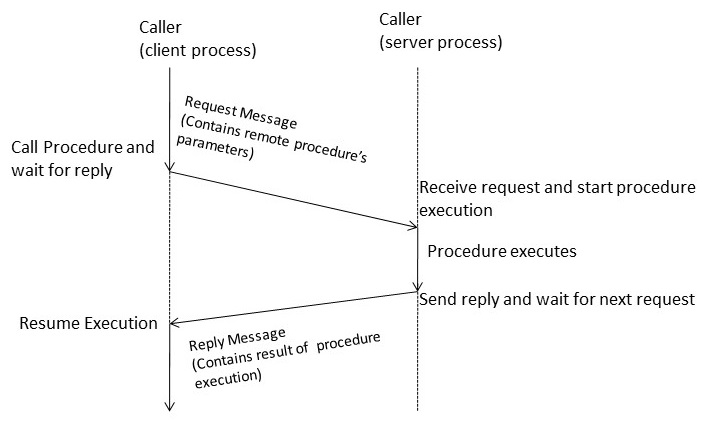
\includegraphics[width=10cm]{fig41.jpg}
	 	\caption{RPC Model}
	 \end{figure}
\end{frame}

\begin{frame}
	\frametitle{Transparency of RPC}
	\justifying{A transparent RPC mechanism is one in which local procedures and remote procedures indistinguishable to the programmers. This requires the following two types of transparencies}
	\vspace{0.2cm}
	\begin{itemize}
		\item Syntactic Transparency
		\item Semantic Transparency
	\end{itemize}
	\vspace{0.5cm}
	- Syntactic transparency are easy\\
	- Semantic Transparency are not easy
	\vspace{3cm}
\end{frame}


\begin{frame}
	\frametitle{Implementation of RPC}
	\justifying{Implementation of RPC mechanism usually involves the following five 
	elements of program.}
	\begin{enumerate}
		\item Client
		\item Client Stub
		\item RPC Run time
		\item Server Stub
		\item Server
	\end{enumerate}
	\vspace{3cm}
\end{frame}

\begin{frame}
	\frametitle{Implementation of RPC...[Cntd..]}
	\begin{figure}
		\centering
		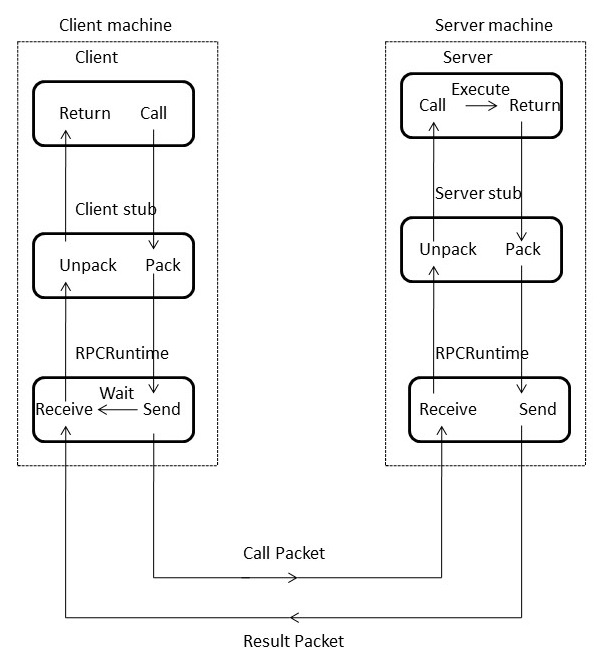
\includegraphics[width=7cm]{fig42.jpg}
		\caption{Implementation of RPC mechanism}
	\end{figure}
\end{frame}


\begin{frame}
	\frametitle{Stub Generation}
	Stub can be generated in one of the following ways.
	\begin{itemize}
		\item Manually
		\item Automatically
	\end{itemize}
	\vspace{6cm}
\end{frame}

\begin{frame}
	\frametitle{RPC Messages}
	There are two types of messages involved in RPC implementation.
	\begin{enumerate}
		\item Call Messages
		\item Reply Messages
	\end{enumerate}
	\vspace{1cm}
	1. Call Message\\
	\begin{figure}
		\centering
		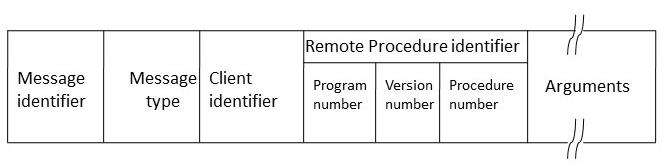
\includegraphics[width=10cm]{fig43.jpg}
		\caption{RPC Call Message Format}
	\end{figure}
\end{frame}


\begin{frame}
	\frametitle{RPC Messages...[Cntd...]}
	\vspace{0.5cm}
	2. Reply Message\\
	\begin{figure}
		\centering
		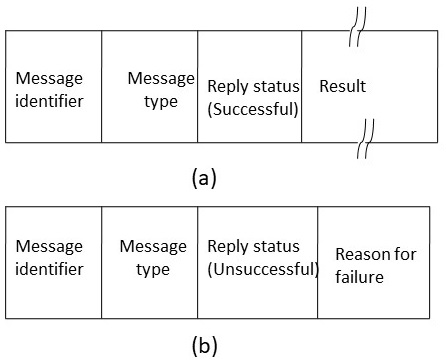
\includegraphics[width=7cm]{fig44.jpg}
		\caption{(a)A Successfule Reply Message Format (b)An Unsuccessful Message Format}
	\end{figure}
\end{frame}

\end{document}